\documentclass[a4paper,11pt]{ltjsarticle}
\usepackage[margin=25mm]{geometry}
\usepackage{amsmath,amssymb}
\usepackage{graphicx}
\usepackage{float}

\title{工学実験 第三回課題}
\author{202025093 安川蒼真}
\date{2026/10/15}

\begin{document}
\maketitle

\section*{課題3.1}
Q学習がどのように進んでいるか，ディスプレイに描画されるエージェントの動きを図\ref{fig:photo1}に添付する．
\begin{figure}[H]
  \centering
  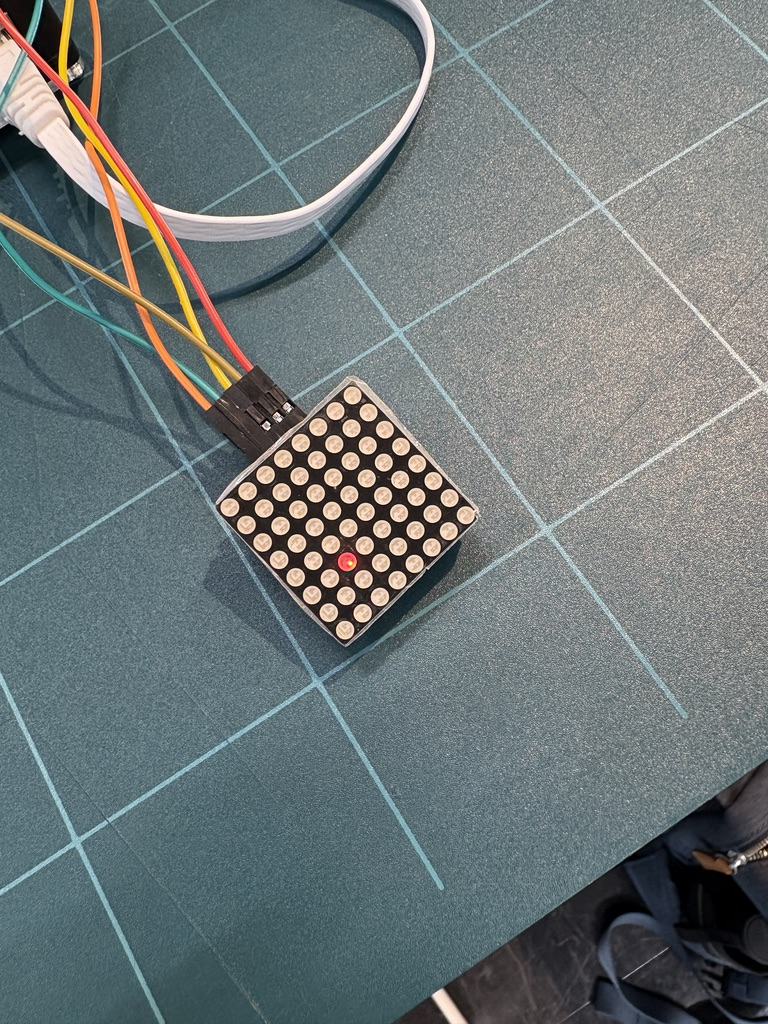
\includegraphics[width=0.3\linewidth]{photos/photo_1.jpeg}
  \caption{Q学習におけるエージェントの動作}
  \label{fig:photo1}
\end{figure}
学習初期には，エージェントが遠回りや同じ場所への移動を
繰り返す様子が見られた．
試行を重ねるにつれて，そのような動作が減少し，
より短い経路でゴールに到達する様子が確認できた．
\section*{課題3.2}
\texttt{exp2\_maze\_ql\_led.py}において，\texttt{terminal=54}および
\texttt{terminal=50}とした場合の，試行回数に対するゴールまでの
ステップ数の変化を，それぞれ図\ref{fig:steps54}，図\ref{fig:steps50}に示す．

\begin{figure}[H]
  \centering
  \begin{minipage}[t]{0.48\linewidth}
    \centering
    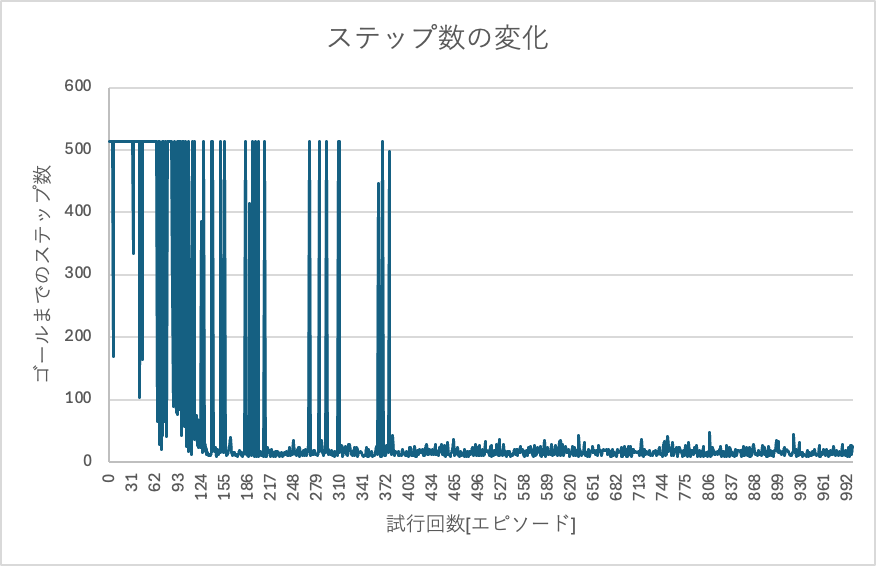
\includegraphics[width=1\linewidth]{figs/3.2_1.png}
    \caption{terminal=54でのステップ数変化}
    \label{fig:steps54}
  \end{minipage}
  \hfill
  \begin{minipage}[t]{0.48\linewidth}
    \centering
    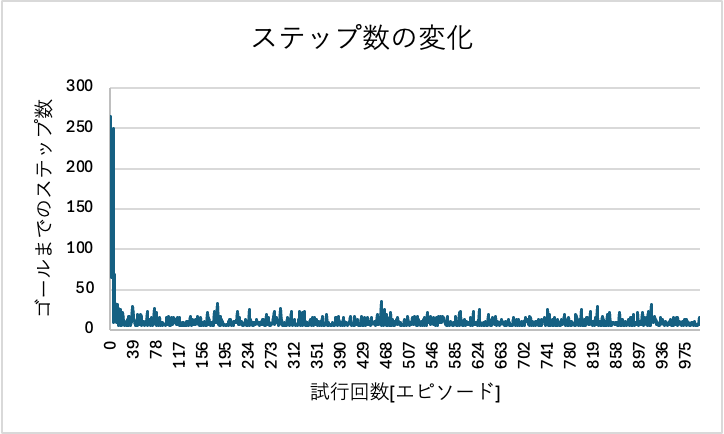
\includegraphics[width=1\linewidth]{figs/3_2_2.png}
    \caption{terminal=50でのステップ数変化}
    \label{fig:steps50}
  \end{minipage}
\end{figure}

\subsection*{考察}
どちらのグラフでも，学習を繰り返すとステップ数が減っている．
ステップ数が少ないということは，ゴールまでに必要な移動回数が
少ないということである．このことから，学習によって遠回りが減り，
より効率よくゴールへ進めるようになったと考えられる．

\texttt{terminal=54}では，初めは約500ステップに達する試行が多く，
約400回目までは，ときどきステップ数が大きく増えている．
一方，\texttt{terminal=50}では，初めは約260ステップだったが，
数十回の試行で大きく減り，その後も少ないステップ数が続いている．
この違いから，今回の実験では\texttt{terminal=50}の方が，
早い段階でゴールへ効率よく進む方法を学習したと考えられる．


\section*{課題3.3}
\texttt{terminal=54}および\texttt{terminal=50}における
学習終了時のQ値マップを，それぞれ図\ref{fig:qmap54}，
図\ref{fig:qmap50}に示す．
いずれの画像も，画面上に\texttt{episode=999}，
\texttt{epsilon=0.30}と表示された時点のものである．

\begin{figure}[H]
  \centering
  \begin{minipage}[t]{0.48\linewidth}
    \centering
    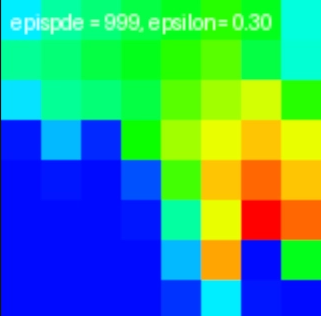
\includegraphics[width=0.8\linewidth]{photos/photo_2.png}
    \caption{terminal=54でのQ値マップ}
    \label{fig:qmap54}
  \end{minipage}
  \hfill
  \begin{minipage}[t]{0.48\linewidth}
    \centering
    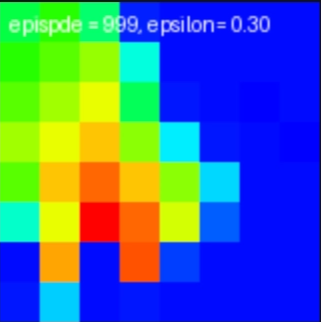
\includegraphics[width=0.8\linewidth]{photos/photo_3.png}
    \caption{terminal=50でのQ値マップ}
    \label{fig:qmap50}
  \end{minipage}
\end{figure}

\subsection*{考察}
2枚のQ値マップを比べると，\texttt{terminal=54}では右側に，
\texttt{terminal=50}では中央から左側に赤色や黄色が多く見られる．
このように，条件を変えると色の分布も変化した．
赤色ほどQ値が大きい表示であれば，赤色の部分には，
高く評価された行動があると考えられる．

Q値は，簡単に言うと「その場所で，その方向へ動くことが，
今後どのくらい報酬につながるか」を表す値である．
ゴールに着くと報酬がもらえる設定なら，例えばゴールの左隣の
マスで右へ動く行動は，すぐに報酬を得られるため，
Q値が大きくなると考えられる．
また，ゴールから離れたマスでも，その先でゴールにつながる行動は，
学習を繰り返すことで高く評価されるようになると考えられる．



\end{document}
